\documentclass[12pt,a4paper]{article}

\usepackage[pdftex]{graphicx}
\usepackage{amsmath,amsopn,amscd,amsthm,amssymb,xypic,rotating}
\usepackage{thmtools}
\usepackage[utf8]{inputenc}
\usepackage{changebar}
\usepackage{tikz}
\usepackage{listings}

\usetikzlibrary{arrows,shapes,positioning,calc}
\usetikzlibrary{decorations.markings}

\tikzstyle{myrectangle} = [draw=black, rectangle,align=center,text width=4cm]
\tikzstyle{myellipse} = [draw=black, ellipse,align=center,text width=3.5cm]


%\tikzstyle arrowstyle=[scale=2]
%\tikzstyle directed=[postaction={decorate,decoration={markings,mark=at position 1 with {\arrow[arrowstyle]{stealth}}}}]
%\tikzstyle bidirected=[postaction={decorate,decoration={markings,mark=at position 1 with {\arrow[arrowstyle]{stealth}}}}]

\newcommand{\tset}[1]      {\{{#1}\}}                     % set data type
\newcommand{\tbag}[1]      {\{\!\!|{#1}\}\!\!\!|}         % bag data type
\newcommand{\tlist}[1]     {[{#1}]}                       %list data type
\newcommand{\ttree}[1]     {{\frak t}({#1})}              %tree data type
\newcommand{\cmd}[1]      {\underline{{#1}}}
\newcommand{\cb}          {\begin{tabbing}MMMMM\=MM\=MM\=MM\=MM\=MM\=MM\=MM\=MM\=MM\= \kill}
\newcommand{\ce}          {\end{tabbing}}
\newcommand{\ontology}[1]	{\ensuremath{\mathcal{#1}}}
\newcommand{\ont}[1]	{\ontology{#1}}
\newcommand{\conceptualization}[1]	{\ensuremath{\mathcal{#1}}}
\newcommand{\conc}[1]	{\conceptualization{#1}}

\newcommand{\HInsert}[2]   {\centerline {\immediate\pdfximage width #2  {#1}\pdfrefximage\pdflastximage}}
\newcommand{\VInsert}[2]   {\centerline {\immediate\pdfximage height #2 {#1}\pdfrefximage\pdflastximage}}


\newtheorem{definition}{Definition}[section]
\newtheorem{proposition}{Proposition}[section]
\newtheorem{corollary}{Corollary}[section]
\newtheorem{theorem}{Theorem}[section]
\newtheorem{lemma}{Lemma}[section]
\newtheorem{statement}{Statement}[section]
\newtheorem{assumption}{Assumption}[section]
\newtheorem{problem}{Problem}[section]

\newcounter{remark}
\newcounter{example}
\setcounter{remark}{0}
\setcounter{example}{0}

\def\example{
\bigskip

\addtocounter{example}{1}%
\noindent \textbf{Example \Roman{example}:}\\
}


\def\remark{
%\addtocounter{remark}{1}%
\refstepcounter{remark}
\noindent \emph{Remark \arabic{remark}:}
}

\renewcommand{\topfraction}{.99}
\renewcommand{\textfraction}{.01}

\newcommand{\dblquote}[1] {\textquotedblleft #1\textquotedblright}

\usepackage{listings}
\usepackage{color}

\definecolor{dkgreen}{rgb}{0,0.6,0}
\definecolor{gray}{rgb}{0.5,0.5,0.5}
\definecolor{mauve}{rgb}{0.58,0,0.82}

\lstset{frame=tb,
  language=Prolog,
  aboveskip=3mm,
  belowskip=3mm,
  showstringspaces=false,
  columns=flexible,
  basicstyle={\small\ttfamily},
  numbers=none,
  numberstyle=\tiny\color{gray},
  keywordstyle=\color{blue},
  commentstyle=\color{dkgreen},
  stringstyle=\color{mauve},
  breaklines=true,
  breakatwhitespace=true,
  tabsize=3
}

\newcommand{\mfunc}[1]      {{\it{#1}}}
\newcommand{\mmfunc}[1]      {\text{\it{#1}}}
\newcommand{\defining}[1] {\emph{#1}}
\newcommand{\keyconcept}[1] {\emph{#1}}
\newcommand{\takeaway}[1] {{\bf{#1}}}
\newcommand{\itemtitle}[1] {{\bf{#1}} - }

\newcommand{\metavars}[1] {\mathcal{#1}}
\newcommand{\unsatmap} {\rightarrow^{\mmfunc{unsat}}}

\newcommand{\objectvar}[1] {\lowercase{#1}}
\newcommand{\metavar}[1] {\uppercase{#1}}
\newcommand{\metametavar}[1] {\mathcal{\uppercase{#1}}}

\title{A few simple tests of performance of meta-resolution}
\author{Juan Casanova}

\begin{document}

\maketitle

\section{About this document}

The aim of this document is to present and analyze a few simple tests of the performance of the implementation of the meta-resolution procedure. These tests are based on a simple working case and extended in different manners to evaluate how the running time of the program scales with these extensions.

\section{Basic example}

The basic example on which the measurements provided in this document is based consists in the detection of provable instantiations of the pattern:

\begin{equation}
\neg \exists x. A
\end{equation}

\noindent in the following ontology:

\begin{equation}
\begin{array}{l}
\forall x. \text{margherita}(x) \implies \text{pizza}(x)\\
\forall x. \text{margherita}(x) \implies \neg (\exists y. \text{hasTopping}(x,y))\\
\forall x. \text{pizza}(x) \implies (\exists y. \text{hasTopping}(x,y)\\
\end{array}
\end{equation}

In CNF, the conjunction of the axioms and the negation of the conjecture consists of the following clauses:

\begin{equation}
\begin{array}{l}
\neg \text{margherita}(x) \lor \text{pizza}(x)\\
\neg \text{margherita}(x) \lor \neg \text{hasTopping}(x,y)\\
\neg \text{pizza}(x) \lor \text{hasTopping}(x,\text{sk}_1(x))\\
A
\end{array}
\end{equation}

\noindent where $\text{sk}_1(x)$ is a Skolem function and meta-variable $A$ may contain Skolem constant $\text{sk}_2$ but no variables.\\

All provable atomic\footnote{Meta-resolution currently only detects atomic instantiations. Extension to composite formulas via inductive instantiation is not implemented yet.} instantiations of the meta-variable $A$ are of the form:

\begin{equation}
A := \text{margherita}(B)
\end{equation}

\noindent for any term $B$. Due to the fact that in the signature provided to the procedure there are no free functions and only the Skolem constant $sk_2$, the only provable instantiation that the procedure may detect is:

\begin{equation}
A := \text{margherita}(sk_2)
\end{equation}

However, different proofs for this same instantiation may be found. This is discussed in more detail in \S \ref{number_solutions}.\\

\subsection{Extending the example}
\label{extending_example}

The way to extend this example to verify the performance behaviour of meta-resolution, as suggested by Alan Bundy, is by introducing intermediate predicates $\text{pizza}_1, \text{pizza}_2, ..., \text{pizza}_n$ and replacing the axiom $\forall x. \text{margherita}(x) \implies \text{pizza}(x)$ for the axioms:

\begin{equation}
\begin{array}{l}
\forall x. \text{pizza}_1(x) \implies \text{pizza}(x)\\
\forall x. \text{pizza}_2(x) \implies \text{pizza}_1(x)\\
...\\
\forall x. \text{margherita}(x) \implies \text{pizza}_n(x)\\
\end{array}
\end{equation}

\noindent or, in CNF, replacing the clause $\text{margherita}(x) \lor \neg \text{pizza}(x)$ for the clauses:

\begin{equation}
\begin{array}{l}
\text{pizza}_1(x) \lor \neg \text{pizza}(x)\\
\text{pizza}_2(x) \lor \neg \text{pizza}_1(x)\\
...\\
\text{margherita}(x) \lor \neg \text{pizza}_n(x)\\
\end{array}
\end{equation}

\section{Parameters controlled}

\subsection{Length of the implication chain}

As explained in \S \ref{extending_example}, we extend the example by introducing intermediate predicates and producing a longer implication chain. This parameter indicates how many intermediate predicates are introduced in each test. We will use the notation $n$ for this parameter.\\

In the results presented here, we have performed measurements for values from $0$ to $7$ for $n$.

\subsection{Maximum depth of proofs attempted}

Meta-resolution currently has an heuristic that allows the user to specify that  any proofs that exceed a certain depth (number of applications of the resolution rule) should be abandoned as improductive. We will use the notation $d$ for this parameter. In principle, lower values of this parameter would prevent the procedure from producing a large number of improductive exploration branches. However, the value needs to be high enough so as to allow the conjecture to be provable. In our particular case, there only exists some proof if $d \geq n+3$.\\

In the results presented here, we have performed measurements for values $5$, $10$, $15$ and $20$ for $d$.

\subsection{Number of solutions}
\label{number_solutions}

While in any of the examples tested there is only one instantiation of the meta-variable that meta-resolution will ever find ($A := \text{margherita}(sk_2)$), there are different proofs for the same instantiation. All of these will be equivalent and their variations will consists mainly in different orders in which the clauses are resolved over and/or adding spurious steps that are not relevant to find the empty clause. However, for the purposes of measuring performance of the procedure and getting an approximate idea of the size of the exploration space, it is useful to allow the procedure to output more solutions and measure the running times. We will use the notation $s$ for this parameter.\\

In the results presented here, we have performed measurements for values $1$, $5$, $10$, $20$ and $50$ for $s$.\\

The number of alternative proofs that there exist for a certain value of $n$ and $d$ is finite, and therefore some combinations of values of $n$, $d$ and $s$ are incompatible due to there being less than $s$ different proofs.

\section{Results and analysis}

The results were measured on my laptop computer. The absolute numbers are not the focus of our investigation, but rather their relatives differences. Results are measured in seconds until the procedure finds up to $s$ different solutions for the problem posed. All the values measured are presented in the following table.

\begin{table}[ht]
\label{all_results}
\caption{Performance times for the different values of $n$, $d$ and $s$. In seconds. The four values in each cell indicate the measurements for $d = 5$, $d = 10$, $d = 15$ and $d = 20$ respectively. $\emptyset$ indicates that not enough solutions were present with that choice of parameters.}
\centering
\begin{tabular}{c | c c | c c | c c | c c | c c |}
&$s=1$&&$s=5$&&$s=10$&&$s=20$&&$s=50$&\\
\hline
$n=0$&0.053&0.043&0.23&0.23&0.52&0.52&1.59&1.59&$\emptyset$&$\emptyset$\\
&0.043&0.046&0.23&0.23&0.51&0.52&1.62&1.6&$\emptyset$&$\emptyset$\\
\hline
$n=1$&0.11&0.12&0.69&0.71&1.41&1.33&3.06&3.36&$\emptyset$&$\emptyset$\\
&0.11&0.12&0.72&0.69&1.4&1.88&3.58&3.5&$\emptyset$&$\emptyset$\\
\hline
$n=2$&0.31&0.36&1.67&1.61&3.5&4&9.32&7.39&$\emptyset$&$\emptyset$\\
&0.38&0.28&1.43&1.44&2.77&2.76&6.8&6.73&$\emptyset$&$\emptyset$\\
\hline
$n=3$&$\emptyset$&0.7&$\emptyset$&3.92&$\emptyset$&7.74&$\emptyset$&15.05&$\emptyset$&48.66\\
&0.52&0.51&2.62&2.6&5.32&5.31&12.9&12.94&48.1&47.77\\
\hline
$n=4$&$\emptyset$&0.96&$\emptyset$&4.84&$\emptyset$&9.96&$\emptyset$&23.48&$\emptyset$&84.73\\
&0.97&0.96&4.85&4.83&9.96&9.93&23.35&23.32&84.62&84.78\\
\hline
$n=5$&$\emptyset$&1.72&$\emptyset$&8.64&$\emptyset$&17.42&$\emptyset$&38.47&$\emptyset$&150.96\\
&1.71&1.72&8.63&8.64&17.46&17.46&38.43&38.5&150.84&150.68\\
\hline
$n=6$&$\emptyset$&2.91&$\emptyset$&14.68&$\emptyset$&29.53&$\emptyset$&60.29&$\emptyset$&254.61\\
&2.92&2.92&14.8&14.62&29.49&29.45&59.95&59.98&254.2&254.39\\
\hline
$n=7$&$\emptyset$&5.01&$\emptyset$&25.29&$\emptyset$&51.03&$\emptyset$&103.36&$\emptyset$&411.72\\
&5.02&5.0&25.31&25.32&51.11&51.11&103.28&103.20&412.06&411.74\\
\hline
\end{tabular}
\end{table}

\subsection{Maximum depth}

One of the first things that are easily noticeable from the results is that the maximum depth parameter $d$ does not have the expected effect on the running times. In almost no case are the running times of the higher maximum depth tests higher than those of the lower maximum depth tests by an amount not totally explainable by experimental randomness and uncontrolled factors such as other programs that may be running on the computer.\\

In fact, in two cases, namely for $n = 3$ when $s \neq 50$, and for $n = 2$ when $s \neq 1$, the running times of the procedure noticeably {\bf{decrease}} when increasing the maximum depth parameter.\\

The explanation is simple: increasing the maximum depth parameter allows the procedure to find longer proofs that it was previously not able to find due to the limitation, and which come earlier in the diagonalization search than latter ones. When the depth increases past the threshold needed for that proof, the procedure finds these solutions considerably earlier because they were a lot earlier in the search. This also explains why for $n = 2$ and $s = 1$ and for $n = 3$ and $s = 50$ the differences vanish: the first proof that the procedure finds for $n = 2$ has less depth than $5$, and so increasing the depth limit has no effect in the time it takes to find it, but subsequent solutions have larger depth and therefore why for $s \neq 1$ the differences are noticeably. Similarly, for $n = 3$, there are likely not many more than $50$ different solutions overall, and so when the procedure is asked to find the $50$ first solutions, the depth limit has little effect as it still needs to traverse most of the search space.\\

\subsection{Length of the implication chain}

The most important insight that we wanted to attain from these tests is an estimation of how the search space grows when the length of the minimum proof grows (length of the implication chain). The answer to this question seems evident from the data: the growth of the search space is exponential on the growth of the implication chain. This becomes evident by plotting the running times for different values of $s$ as a function of $n$ in logarithmic scale. See figure \ref{n_to_time}. Not only are all of these relations exponential, but also they seem to have the same base, independent of $s$, as clear by the fact that the slope in logarithmic scale is the same for all of them. More precise calculations seem to indicate that this base (slope) seems to be between $1.65$ and $1.9$, and slightly decrease with $n$ and with $s$. That is, it seems that the running time $t$ as a function of $n$ has an expression of the form $t(n) = k \cdot 1.75^{n}$, approximately.

\begin{figure}
\centering
\caption{\label{n_to_time}Relation between $n$ and running time for different values of $s$. $d = 15$. Logarithmic scale.}
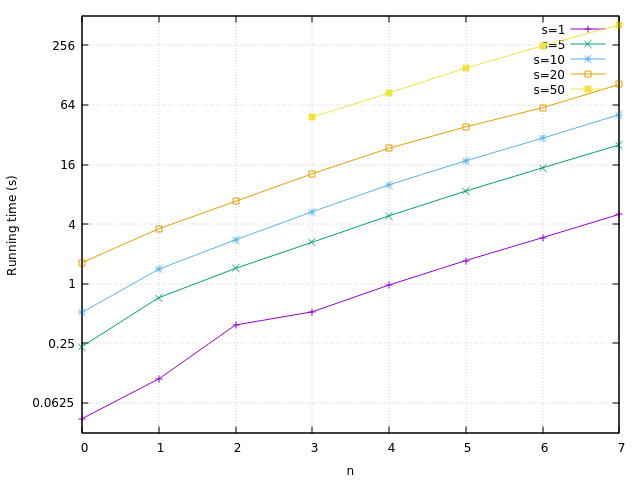
\includegraphics[width=1\textwidth]{n_to_time.png}
\end{figure}

\subsection{Number of solutions}

It is also relevant to consider how requesting more solutions to the procedure affects the running time. The relation seems to be slightly more increasing than linear, as can be observed from figure \ref{s_to_time}. That is, obtaining the next solution tends to be slightly more expensive than the last one that we just obtained.\\

While it is hard to extract any clear conclusions from this information at this point, considering that the diagonalization procedure makes the search grow both in breadth and in depth as it goes on, these data seem to indicate that solutions are relatively evenly spread throughout the search space, and the increased running time between each solution could be due to the increase in breadth of the search space (number of branches kept alive at the same time). However, it is also possible that this could be explained by solutions tending to appear more towards the beginning of the search space.\\

The most important conclusion we can extract from this, however, is that the quasi-linear growth of the running time with the number of solutions hints that the breadth growth of the search space is, in general, productive, and that it is not the case that the number of potential solutions explored grows considerably quicklier than the number of those that are actual solutions. That is, the amount of improductive search does not considerably increase during the execution of the procedure, and therefore should not, in principle, be a cause for concern.

\begin{figure}
\centering
\caption{\label{s_to_time}Relation between $s$ and running time for different values of $n$. $d = 15$. Other values of $n$ have similar relations and have been omitted for clarity of the plot.}
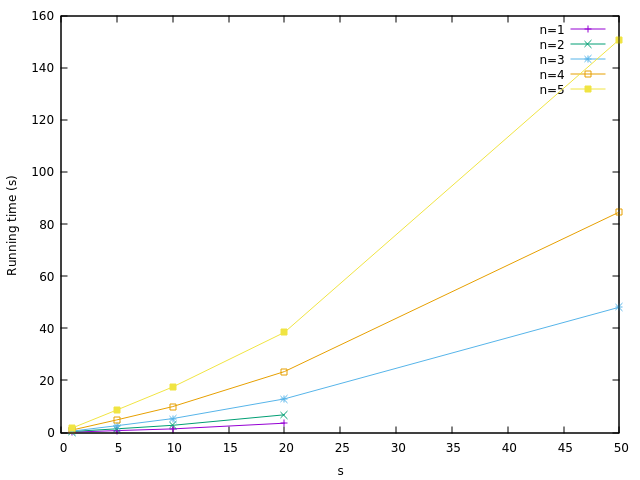
\includegraphics[width=1\textwidth]{s_to_time.png}
\end{figure}

\section{Limitations of the analysis}

The analysis presented here is highly preliminary and clearly has important limitations.\\

First and perhaps most importantly, the choice of a specific and highly regular family of problems to evaluate (implication chains). It is unclear if this regularity could be masking phenomena that appear on other, more complicated, proofs and that are relevant for the performance of the procedure.\\

Second, the inability to measure other relevant quantities in the runs of the procedure due to the current state of the program. For example, it would be enlightening to know what the total breadth of the search space is at each point during the search (how many potential different solutions are being evaluated at the same time), and how this number correlates with the number of solutions found and with the running time. Similarly and in close relation, it would be interesting to know how many solutions are discarded as invalid for our problem in relation to the breadth of the search and the number of valid solutions found.\\

Third, the limited sample. The number of data points offered here are not enough to draw conclusive insights, even on the limited choice of problems. However, the high regularity and clear tendencies found in the results obtained   seem to indicate that the limited sample might not be the biggest of issues in this case.\\

Finally, the inability to relevantly control factors of how the procedure runs. While there are some possibilities for heuristics to be included (and are included) in the procedure, they are primitive and do not produce a very relevant difference in the running times of the procedure. Being able to fine tune how many steps in each proof are carried out before branching out to a new potential solution or limiting or guiding the meta-variable instantiations explored could prove to be critical factors for the performance of the procedure.\\

\end{document}